%%%%%%%%%%%%%%%%%%%%%%%%%%%%%%%%%%%%%
%%%%%%%%%%%%            PREAMBLE          %%%%%%%%%%%%
%%%%%%%%%%%%%%%%%%%%%%%%%%%%%%%%%%%%%

\documentclass[aspectratio=169, xcolor=dvipsnames]{beamer}
\usecolortheme[named=Red]{structure} 
\usepackage{graphicx}
\usepackage{subcaption}

%%%%%%%%%%%%%%%%%%%%%%%%%%%%%%%%%%%%
%%%%%%%%%%%%           TITLE PAGE         %%%%%%%%%%%
%%%%%%%%%%%%%%%%%%%%%%%%%%%%%%%%%%%%

\title[]{Poverty Mapping in the Age of Machine Learning}

\date{\today}

\author[]{Paul Corral, Heath Henderson, and Sandra Segovia}



\begin{document}

%%%%%%%%%%%%%%%%%%%%%%%%%%%%%%%%%%%%
%%%%%%%%%%%%%           CONTENT         %%%%%%%%%%%
%%%%%%%%%%%%%%%%%%%%%%%%%%%%%%%%%%%%

% Title slide
\begin{frame}
\titlepage
\end{frame}

% Introduction
\begin{frame}{Introduction}
\begin{itemize}
\item Poverty maps provide granular estimates of poverty at the sub-national level.
\par\pause\noindent
\item Poverty mapping typically requires small area estimation, which consists of 
two basic steps:
\begin{enumerate}
\item Fit a statistical model using household survey data
\item Apply the model to census data to predict poverty rates
\end{enumerate}
\par\pause\noindent
\item Traditional approaches rely on parametric statistical models applied 
to population census data.
\par\pause\noindent
\item There are a wide variety of traditional approaches, including unit-level,
unit-context, and area-level models.
\end{itemize}
\end{frame}

% Introduction
\begin{frame}{Introduction}
\begin{itemize}
\item The modern approach consists of several practices that differ from the 
traditional approach:
\begin{enumerate}
\item Non-parametric statistical methods
\item Remotely-sensed data
\item Validation procedure based on $R^2$
\end{enumerate}
\par\pause\noindent
\item $R^2$ is calculated by regressing direct, survey-based poverty estimates 
on the model-based predictions.
\par\pause\noindent
\item While direct estimates are unbiased, they can be imprecise estimates of 
true poverty measures.
\par\pause\noindent
\item In this paper, we provide a more rigorous assessment of the modern 
approach to poverty mapping.
\end{itemize}
\end{frame}

% Introduction
\begin{frame}{An Example}
% Note: Yeh et al. use data from 23 African countries. Data is at the level of the
% enumeration area, which they call "villages."
\begin{minipage}{0.5\textwidth}
\begin{figure}[h]
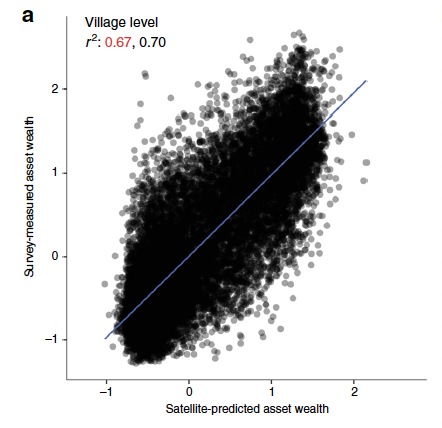
\includegraphics[width=0.75 \textwidth]{Yeh}
\end{figure}
\end{minipage} \hfill
\begin{minipage}{0.45\textwidth}
``These results exceed performance in earlier work on a
similar task using high-resolution imagery or mobile phone
data as input, and match or exceed benchmarks for in-country
performance from geostatistical models used to predict health
outcomes, standard of living, and housing quality in Africa'' (Yeh et al.\ 2020)
\end{minipage}
\end{frame}

% Data
\begin{frame}{Data}
\begin{itemize}
\item We use the 2015 Mexican Intercensal Survey to construct a ``census'' that 
we use to conduct simulation experiments.
\par\pause\noindent
\item The census consists of 3.9 million households across 1,865 municipalities and
16,297 PSUs.
\par\pause\noindent
\item For each household, we observe income, geographic location, demographics,
and dwelling characteristics, among other information.
\par\pause\noindent
\item We supplement the census data with remotely-sensed data available at the
municipality level:
\begin{itemize}
\item 105 different indicators (21 different dimensions)
\item Example dimensions include measures related to vegetation, urbanization,
water, and altitude
\end{itemize}
\end{itemize}
\end{frame}

% Data
\begin{frame}{Data}
\begin{itemize}
\item We draw 500 survey samples ($\approx$ 23,500 households each) from the 
census using a two-stage design:
\begin{enumerate}
\item We select PSUs with probability proportional to size
\item We select 10 households within each cluster
\end{enumerate}
\par\pause\noindent
\item For each sample, we then have direct poverty estimates and 
true poverty measures for each subnational entity.
\par\pause\noindent
\item We implement several different approaches to poverty mapping using the 
survey datasets:
\begin{itemize}
\item Parametric versus non-parametric models
\item PSU-level versus municipality-level estimation
\item Census-based versus remotely-sensed covariates
\end{itemize}
\end{itemize}
\end{frame}

% Machine Learning
\begin{frame}{Machine Learning}
\begin{itemize}
\item We focus on one particularly popular machine-learning method: gradient 
boosting.
\par\pause\noindent
\item Originally developed by Friedman (2001), gradient boosting combines a 
large number of weak learners to form a stronger ensemble prediction.
\par\pause\noindent
\item Rather than averaging models, gradient boosting sequentially adds models 
(trees) to the ensemble by fitting new models to negative gradient of the loss function:
\begin{equation*}
y_i^p = \sum_t f_t(x_i)
\end{equation*}
\par\pause\noindent
\item We specifically use extreme gradient boosting (XGBoost) where each tree
is built by minimizing the following regularized objective function: 
\begin{equation*}
\mathcal{L} = \sum_i l(y_i^d, y_i^p) + \sum_t r(f_t)
\end{equation*}
\end{itemize}
\end{frame}

% Machine Learning
\begin{frame}{Machine Learning}
\begin{figure}
\begin{subfigure}[h]{0.4\linewidth}
\includegraphics[width=\linewidth]{tree}
\caption{Regression tree}
\end{subfigure}
\hspace{10pt}
\begin{subfigure}[h]{0.4\linewidth}
\includegraphics[width=\linewidth]{partition}
\caption{Covariate space}
\end{subfigure}
\end{figure}
\end{frame}

% Traditional Methods
\begin{frame}{Traditional Methods}
\begin{itemize}
\item We consider three alternative traditional methods: 
unit-level, unit-context, and area-level models.
\par\pause\noindent
\item The unit-level model is typically considered the ``gold standard'' of
traditional poverty mapping:
\begin{equation*}
w_{iv} = x_{iv} \theta + \mu_i + \xi_{iv}
\end{equation*}
\par\pause\noindent
\item The parameters of the model are used to generate $K$ income
estimates for each household in the census:
\begin{equation*}
\hat{w}_{ivk} = x_{iv} \hat{\theta} + \mu^*_i + \xi^*_{iv}
\end{equation*}
\par\pause\noindent
\item The unit-level model is a useful benchmark, but is not a direct competitor
to modern approaches.
\end{itemize}
\end{frame}

% Traditional Methods
\begin{frame}{Traditional Methods}
\begin{itemize}
\item The unit-context model is an alternative traditional method that was 
designed to be used with out-of-date census data.
\par\pause\noindent
\item Rather than using household-level covariates $x_{iv}$, the unit-context
model simply substitutes census aggregates $x_i$.
\par\pause\noindent
\item The area-level model is yet another alternative that models area-level 
poverty rates directly as a function of area aggregates.
\par\pause\noindent
\item Both the unit-context and area-level models can be viewed as direct 
competitors to the modern approach to poverty mapping.
\end{itemize}
\end{frame}

% Model Validation
\begin{frame}{Model Validation}
\begin{itemize}
\item The standard method for assessing performance calculates $R^2$ as follows:
\begin{equation*}
y_i^d = \alpha + \delta y_i^p + \zeta_i \hspace{10pt} \Rightarrow
\hspace{10pt} R_d^2 = \frac{\sigma_d^2 - \sigma_\zeta^2}{\sigma_d^2}
\end{equation*}
\par\pause\noindent
\item Model-based predictions are more appropriately assessed as follows:
\begin{equation*}
y_i^a = \alpha + \delta y_i^p + \upsilon_i \hspace{10pt} \Rightarrow
\hspace{10pt} R_a^2 = \frac{\sigma_a^2 - \sigma_\upsilon^2}{\sigma_a^2}
\end{equation*}
\par\pause\noindent
\item Let $y_i^d = y_i^a + \omega_i$ and let $B = R_a^2 -  R_d^2$. We can then write
\begin{equation*}
R_d^2 = R_a^2 \left(\frac{\sigma_d^2 - \sigma_\omega^2}{\sigma_d^2} \right)
\end{equation*}
\end{itemize}
\end{frame}

% Model Validation
\begin{frame}{Model Validation}
\begin{itemize}
\item An arguably better approach is to calculate the mean squared error directly:
\begin{equation*}
\text{MSE}(y_i^a, y_i^p) = \frac{1}{N} \sum_i (y_i^a - y_i^p)^2
\end{equation*}
\par\pause\noindent
\item With multiple estimates for each entity, we can write the following:
\begin{equation*}
\text{MSE}_i = \frac{1}{K} \sum_k (y_i^a - y_{ik}^p)^2 
=  \frac{1}{K}\sum_k (y_{ik}^p - \bar{y}_i^p)^2 + (\bar{y}_i^p - y_i^a)^2
\end{equation*}
\par\pause\noindent
\item With the above, we can assess the MSE for different entities and examine
both the variance and bias associated with the predictions.
\end{itemize}
\end{frame}

% Model Validation
\begin{frame}{Model Validation}
\begin{enumerate}
\small
\item Using the true household-level incomes, calculate the poverty headcount and 
poverty gap for the country as a whole for some chosen poverty line. 
Using the poverty gap measure, determine the budget required to completely 
eradicate poverty. Calculate an individual-level transfer amount by dividing the 
total budget by the number of people living in poverty. 
\par\pause\noindent
\item Using a given poverty map, order the geographical entities according to their 
estimated poverty headcounts, from most to least poor. 
For the poorest region, augment the true per capita income of all households by 
an amount equal to the transfer. 
Continue this distribution procedure for the second poorest region, the third poorest 
region, and so on until there are not enough resources to cover all households in a 
given region. 
For the marginal region, distribute the remaining budget equally among individuals in 
that region.
\par\pause\noindent
\item Using the post-transfer household incomes, calculate an updated poverty 
headcount to assess the effects of the distribution scheme on poverty alleviation.
\end{enumerate}
\end{frame}

% Results
\begin{frame}{Results}
% Note: The direct R-squared identifies the incorrect level of estimation for 
% 87 percent of the samples.
\begin{figure}[h!]
  \centering
  
\includegraphics[width=0.6 \textwidth]{Figure-1a}
\end{figure}
\end{frame}

% Results
% Note: The median root MSE for gradient boosting (GIS-MUN) is about 0.09,
% meaning the median error is about 9 percentage points.
\begin{frame}{Results}
\begin{figure}[h!]
  \centering
  
\includegraphics[width=0.6 \textwidth]{Figure-2a}
\end{figure}
\end{frame}

% Results
% Note: The minimum and maximum bias for gradient boosting (GIS-MUN) is
% -0.43 and 0.43, respectively. 
\begin{frame}{Results}
\begin{figure}[h!]
  \centering
  
\includegraphics[width=0.6 \textwidth]{Figure-2b}
\end{figure}
\end{frame}

% Results
% Note: All of the top 10 covariates are census-based and only five geo-referenced
% covariates enter the top 20.
\begin{frame}{Results}
\begin{figure}[h!]
  \centering
  
\includegraphics[width=0.6 \textwidth]{Figure-3}
\end{figure}
\end{frame}

% Results
\begin{frame}{Results}
\begin{figure}[h!]
  \centering
  
\includegraphics[width=0.6 \textwidth]{Figure-6}
\end{figure}
\end{frame}

% Conclusions
\begin{frame}{Conclusions}
\begin{itemize}
\item The results of our simulations can be summarized as follows:
\begin{enumerate}
\item The direct $R^2$ exhibits considerable downward bias, with the true $R^2$ 
being roughly 35 to 50 percent higher.
\item The modern approach to poverty mapping performs relatively poorly in terms
of mean squared error and bias.
\item We also found that the modern approach exhibits relatively poor performance
in our targeting simulations.
\end{enumerate}
\par\pause\noindent
\item Main takeaway: The type of covariate information used for poverty mapping 
appears to be more critical than the statistical method.
\par\pause\noindent
\item Limitation: It is possible that the remotely-sensed data we use has less 
predictive power than the data used in other applications.
\end{itemize}
\end{frame}

\end{document}


















